% Insert HW number and date into heading!

\documentclass[10pt]{article}
\usepackage[margin=1in]{geometry}
%\addtolength{\oddsidemargin}{-.1in} 
\usepackage{amsmath,amsthm,amssymb}
\usepackage{bm}
\usepackage{enumitem}
\usepackage{array}
\usepackage{lipsum}
\usepackage[]{units}
\usepackage{relsize}
\usepackage{verbatim}
\usepackage{mathrsfs}

\usepackage{tikz}
\usetikzlibrary{positioning}
\usepackage{graphicx}
\usepackage{xfrac}

\setenumerate{listparindent=\parindent}

\newcommand{\N}{\mathbb{N}}
\newcommand{\Z}{\mathbb{Z}}
\newcommand{\Q}{\mathbb{Q}}
\newcommand{\R}{\mathbb{R}}
\newcommand{\C}{\mathbb{C}}
\newcommand{\D}{\mathbb{D}}
\newcommand{\U}{\mathcal{U}}
\newcommand{\Int}{\displaystyle\int}

\DeclareMathOperator*{\dom}{dom}
\DeclareMathOperator*{\re}{Re}
\DeclareMathOperator*{\im}{Im}
\DeclareMathOperator*{\res}{res}
\DeclareMathOperator*{\PV}{PV}
\renewcommand{\bar}{\overline}
%\renewcommand{\int}{\int}

\definecolor{mygray}{rgb}{.8,.8,0.8}

\newtheorem*{lem}{Lemma}

%%% Heading %%%

\usepackage{fancyhdr}
\pagestyle{fancy}
\lhead{Math 185 (HW 7)}
\chead{Michael Knopf (24457981)}
\rhead{August $12^{\text{th}}$, 2015}
\lfoot{}
\cfoot{}
\rfoot{}
\renewcommand\headrulewidth{0.4pt}

\begin{document}

\begin{enumerate}
\setcounter{enumi}{52}

\item Let $\Gamma$ be the cycle shown in the figure.  Compute the winding numbers of $\Gamma$ in each connected component of $\Gamma \setminus \C$.
\begin{figure}[ht!]
\centering
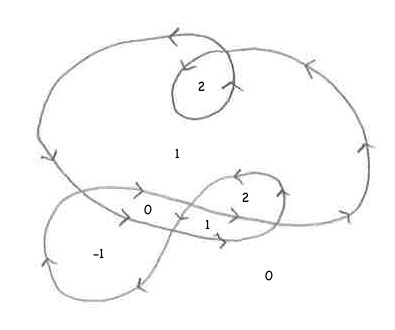
\includegraphics[width=120mm]{winding1.jpg}
\end{figure}

\item Let $\Gamma$ be the cycle shown in the figure.  Compute the winding numbers of $\Gamma$ in each connected component of $\Gamma \setminus \C$.
\begin{figure}[ht!]
\centering
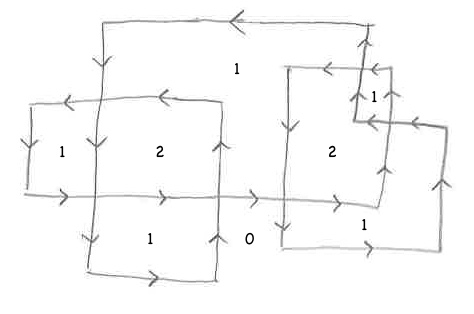
\includegraphics[width=120mm]{winding2.jpg}
\end{figure}

\pagebreak
\item $\Int_0^{\frac{\pi}{2}} \frac{1}{a + \sin^2 x} dx$, \hspace{.5cm} $|a| > 1$

\begin{proof}
Let $C$ be the unit circle.  This integral can be expressed as
$$
\Int_0^{\frac{\pi}{2}} \frac{1}{a + \sin^2 x} dx = \frac{1}{4}\Int_0^{2\pi} \frac{1}{a + \sin^2 x} dx = \frac{1}{4} \Int_{C} \frac{1}{a + (\frac{z - z^{-1}}{2i})^2} \frac{1}{iz} dz = i \int_{C} \frac{z}{z^4 - 2(1+2a)z^2 + 1} dz.
$$
The roots of the integrand's denominator are below.
$$
z_1 = + \sqrt{(1+2a) +2 \sqrt{a^2 + a}} \hspace{1cm}
z_2 = - \sqrt{(1+2a) +2 \sqrt{a^2 + a}}
$$
$$
z_3 = + \sqrt{(1+2a) -2 \sqrt{a^2 + a}} \hspace{1cm}
z_4 = - \sqrt{(1+2a) -2 \sqrt{a^2 + a}}
$$
Now, $z_j$ is a singularity if and only if $|z_j| < 1$.  We can determine when this occurs as follows:
$
|z_j| = \left| \pm \sqrt{(1+2a) \pm 2 \sqrt{a^2 + a}} \right| < 1
$
if and only if
$$
\left| (1+2a) \pm 2 \sqrt{a^2 + a}\right| = \left| \pm \sqrt{(1+2a) \pm 2 \sqrt{a^2 + a}} \right|^2 < 1.
$$
Currently, it is still possible that the expression in the absolute values on the left is negative.  We can square it again to ensure the resulting expression is positive:
$$
(8a^2 + 8a + 1) \pm 4(1+2a)\sqrt{a^2 + a} = \left| (1+2a) \pm 2 \sqrt{a^2 + a}\right|^2 < 1
$$
$$
\iff 8(a^2 + a) \pm 4(1+2a)\sqrt{a^2 + a} < 0.
$$
Regardless of the value of $a$, we know $a^2 + a > 1 + 1 > 0$.  So we can divide both sides of the inequality by $4\sqrt{a^2 + a}$ to obtain
$$
2\sqrt{a^2 + a} \pm (1+2a) < 0
$$
as a necessary and sufficient condition for $z_j$ to be a singularity.  Clearly, the only way to satisfy this inequality is for the $\pm$ to be taken as $+$ when $a < 1$, or the $\pm$ to be taken as $-$ when $a > 1$.  In the first case, the lefthand side can be expressed as
$$
2\sqrt{a^2 + a} + (1+2a) = 2\sqrt{a^2 + a} - |1+2a|
$$
reducing the inequality to $2\sqrt{a^2 + a} < |1+2a|$.  Since both sides are positive, squaring them gives an equivalent expression.  However, this resulting expression is an identity, thus $z_1$ and $z_2$ are poles when $a < -1$.  When $a > 1$, the same argument shows that $z_3$ and $z_4$ are poles.  Therefore, letting $f(z) = \dfrac{z}{z^4 - 2(1+2a)z^2 + 1} = \dfrac{z}{(z - z_1) (z - z_2) (z - z_3) (z - z_4)}$, we have
$$
i \int_{C} f(z) dz =
\begin{cases}
-2\pi [\res\nolimits_{z_1} f(z) + \res\nolimits_{z_2} f(z) ] & \text{ if } a < -1 \\
-2\pi [\res\nolimits_{z_3} f(z) + \res\nolimits_{z_4} f(z) ] & \text{ if } a > 1
\end{cases}.
$$
\end{proof}
All four of the poles are simple.  For convenience, let $\alpha = 1+2a$ and $\beta = \sqrt{a^2 + a}$.  Note that $z_1 = - z_2$, $z_3 = - z_4$, and $z_1z_3 = z_2z_4 = 1$.  We compute the residues as
\begin{align*}
\res\nolimits_{z_1} f(z) &= \lim_{z \rightarrow z_1} (z - z_1) \dfrac{z}{(z - z_1) (z - z_2) (z - z_3) (z - z_4)}
\\
&= \dfrac{z_1}{(z_1 - z_2) (z_1 - z_3) (z_1 - z_4)}
= \dfrac{z_1}{2z_1 (z_1 - z_3) (z_1 - z_4)}
= \dfrac{1}{2[z_1^2 - z_1(z_3 + z_4) + z_3z_4]}
\\
&= \dfrac{1}{2[z_1^2 + z_3z_4]}
= \dfrac{1}{2[(\alpha + 2 \beta) - (\alpha - 2\beta)]}
= \dfrac{1}{8\beta}
= \boxed{\frac{1}{8\sqrt{a^2 + a}}}
\\
%%%%%%%%%%%%%%%%%%%%%%%
%%%%%%%%%%%%%%%%%%%%%%%
\res\nolimits_{z_2} f(z) &= \lim_{z \rightarrow z_2} (z - z_2) \dfrac{z}{(z - z_1) (z - z_2) (z - z_3) (z - z_4)}
\\
&= \dfrac{z_2}{(z_2 - z_1) (z_2 - z_3) (z_2 - z_4)}
= \dfrac{z_2}{2z_2(z_2 - z_3) (z_2 - z_4)}
= \dfrac{1}{2[z_2^2 - z_2(z_3 + z_4) + z_3z_4]}
\\
&= \dfrac{1}{2[z_2^2 + z_3z_4]}
= \dfrac{1}{2[(\alpha + 2 \beta) - (\alpha - 2\beta)]}
= \dfrac{1}{8\beta}
= \boxed{\frac{1}{8\sqrt{a^2 + a}}}
%%%%%%%%%%%%%%%%%%%%%%%
%%%%%%%%%%%%%%%%%%%%%%%
\\
\res\nolimits_{z_3} f(z) &= \lim_{z \rightarrow z_3} (z - z_3) \dfrac{z}{(z - z_1) (z - z_2) (z - z_3) (z - z_4)}
\\
&= \dfrac{z_3}{(z_3 - z_1) (z_3 - z_2) (z_3 - z_4)}
= \dfrac{z_3}{2z_3(z_3 - z_1) (z_3 - z_2)}
= \dfrac{1}{2[z_3^2 - z_3(z_1 + z_2) + z_1z_2]}
\\
&= \dfrac{1}{2[z_3^2 + z_1z_2]}
= \dfrac{1}{2[(\alpha - 2 \beta) - (\alpha + 2\beta)]}
= -\dfrac{1}{8\beta}
= \boxed{-\frac{1}{8\sqrt{a^2 + a}}}
%%%%%%%%%%%%%%%%%%%%%%%
%%%%%%%%%%%%%%%%%%%%%%%
\\
\res\nolimits_{z_4} f(z) &= \lim_{z \rightarrow z_4} (z - z_4) \dfrac{z}{(z - z_1) (z - z_2) (z - z_3) (z - z_4)}
\\
&= \dfrac{z_4}{(z_4 - z_1) (z_4 - z_2) (z_4 - z_3)}
= \dfrac{z_4}{2z_4(z_4 - z_1) (z_4 - z_2)}
= \dfrac{1}{2[z_4^2 - z_4(z_1 + z_2) + z_1z_2]}
\\
&= \dfrac{1}{2[z_4^2 + z_1z_2]}
= \dfrac{1}{2[(\alpha - 2 \beta) - (\alpha + 2\beta)]}
= -\dfrac{1}{8\beta}
= \boxed{-\frac{1}{8\sqrt{a^2 + a}}}
\end{align*}
Finally, we have
$$
\boxed{
\Int_0^{\frac{\pi}{2}} \frac{1}{a + \sin^2 x} dx
=
\begin{cases}
- \dfrac{\pi}{2 \sqrt{a^2 + a}}& \text{ if } a < -1 \vspace{.2cm} \\
\dfrac{\pi}{2 \sqrt{a^2 + a}}& \text{ if } a > 1
\end{cases}}
$$


\item $\Int_0^\pi \dfrac{\cos 2\theta}{1 - 2a \cos\theta + a^2} d\theta$, \hspace{.5cm}  $-1 < a < 1$

\begin{proof}
If $a=0$ then this integral is simply 0.  So we may assume that $a \neq 0$.  Notice that the integrand is symmetric about $\pi$, since $\cos$ is symmetric about both $\pi$ and $2\pi$.  So, letting $C$ be the unit circle, we have
\begin{align*}
\Int_0^\pi \dfrac{\cos 2\theta}{1 - 2a \cos\theta + a^2} d\theta
&= \frac{1}{2} \Int_0^{2\pi} \dfrac{\cos 2\theta}{1 - 2a \cos\theta + a^2} d\theta
= \frac{1}{2} \int_C \frac{\frac{z^2 + z^{-2}}{2}}{1 - 2a\frac{z + z^{-1}}{2} + a^2} \frac{1}{iz} dz
\\
&= -\frac{1}{4ai} \int_C \frac{z^4 + 1}{z^2[az^2 - (a^2+1)z + a]} dz = -\frac{1}{4ai} \int_C \frac{z^4 + 1}{z^2(z-a)(z-\frac1a)} dz
\end{align*}
thus there is a pole of order $2$ at $z_0 = 0$ and a simple pole at $z_1 = a$, since $|\frac{1}{a}| > 1$.  We compute the residues as
\begin{align*}
\res\nolimits_{0} &= \lim_{z \rightarrow 0 } \frac{1}{1!}\frac{d}{dz} z^2 \frac{z^4 + 1}{z^2(z-a)(z-\frac{1}{a})}
=
a + \frac1a
\\
\res\nolimits_{a} &= \lim_{z \rightarrow a} \frac{1}{0!} (z-a)\frac{z^4 + 1}{z^2(z-a)(z-\frac{1}{a})} = \frac{a^4 + 1}{a^2(a-\frac1a)}
\end{align*}
Therefore,
$$
\Int_0^\pi \dfrac{\cos 2\theta}{1 - 2a \cos\theta + a^2} d\theta
=
-\frac{2\pi i}{4ai} \left[\left(a + \frac1a \right) + \frac{a^4 + 1}{a^2(a-\frac1a)} \right]
=
 \dfrac{\pi a^2}{1-a^2}
$$
when $a \neq 0$.  Therefore,
$$
\boxed{
\Int_0^\pi \dfrac{\cos 2\theta}{1 - 2a \cos\theta + a^2} d\theta
\begin{cases}
0 & \text{ if } a = 0 \\
 \dfrac{\pi a^2}{1-a^2} & \text{ if } a \neq 0
\end{cases}
}
$$
\end{proof}

\item $\Int_0^\infty \frac{x^2}{x^4 + 5x^2 + 6} dx$

\begin{proof}
Consider the integral $\Int_{-\infty}^\infty \frac{x^2}{x^4 + 5x^2 + 6} dx$.  This integral satisfies the conditions in the example done in lecture: the denominator is a polynomial of degree at least 2 more than that of the numerator with no roots on the real axis.  The only poles on the positive imaginary axis are $x = \sqrt{2} i$ and $x = \sqrt{3}i$.  We compute these residues as
\begin{align*}
\res\nolimits_{\sqrt{2} i} &= \lim_{z \rightarrow \sqrt{2} i} (z - \sqrt{2} i) \frac{z^2}{z^4 + 5z^2 + 6} = \lim_{z \rightarrow \sqrt{2} i} \dfrac{z^2}{(z + \sqrt{2}i)(z^2 + 3)} = \dfrac{-2}{2\sqrt{2}i(-2 + 3)} = - \dfrac{1}{\sqrt{2}i}
\\
\res\nolimits_{\sqrt{3} i} &= \lim_{z \rightarrow \sqrt{3} i} (z - \sqrt{3} i) \frac{z^2}{z^4 + 5z^2 + 6} = \lim_{z \rightarrow \sqrt{3} i} \dfrac{z^2}{(z + \sqrt{3}i)(z^2 + 2)} = \dfrac{-3}{2\sqrt{3}i(-3 + 2)} = \dfrac{\sqrt{3}}{2i}
\end{align*}

Since the integrand is an even function, we have
\begin{align*}
\Int_{0}^\infty \frac{x^2}{x^4 + 5x^2 + 6} dx &= \frac12 \Int_{-\infty}^\infty \frac{x^2}{x^4 + 5x^2 + 6} dx
= \frac{2\pi i}{2}\left[ \dfrac{\sqrt{3}}{2i} - \dfrac{1}{\sqrt{2}i} \right] = \boxed{\frac{\pi(\sqrt{3} - \sqrt{2})}{2}}
\end{align*}
\end{proof}

\item $\PV \Int_{-\infty}^{\infty} \dfrac{1}{(x^2 - 1)(x^2 + 2x + 2)}dx$

\begin{proof}
Let $f(z) = \dfrac{1}{(z^2 - 1)(z^2 + 2z + 2)}$.  The principal value of this integral is
$$
\PV \Int_{-\infty}^{\infty} f(x)dx
=
\lim_{\epsilon \rightarrow 0} \left( \int_{-\infty}^{-1-\epsilon} f(z) dz + \int_{-1+ \epsilon}^{1 - \epsilon} f(z) dz + \int_{1+\epsilon}^\infty f(z) dz \right).
$$
Let $\Gamma_{R,\epsilon}$ be the curve made up of a semicircle of radius $R$ centered at $0$, and a line segment connecting its ends along the real axis that cut out the singularities at $z = \pm 1$ with semicircles of radius $\epsilon$.  Then
$$
\lim_{\epsilon \rightarrow 0} \left( \int_{-\infty}^{-1-\epsilon} f(z) dz + \int_{-1+ \epsilon}^{1 - \epsilon} f(z) dz + \int_{1+\epsilon}^\infty f(z) dz \right) = \lim_{\substack{\epsilon \rightarrow 0 \\ R \rightarrow \infty}} \int_{\Gamma_{R,\epsilon}} f(z) dz.
$$
By Lemma IV.3.3, this equals
$$
2\pi i \sum_{\im (z) > 0} \res\nolimits_z [f(z)] + \pi i \sum_{\im (z) = 0} \res\nolimits_z [f(z)].
$$
The only singularities we are concerned with are $-1, +1,$ and $-1 + i$, of which all are simple poles.  We compute each residue as
\begin{align*}
\res\nolimits_{-1}[f(z)] &= \lim_{z \rightarrow -1} (z+1)\dfrac{1}{(z^2 - 1)(z^2 + 2z + 2)} = \lim_{z \rightarrow -1} \dfrac{1}{(z - 1)(z^2 + 2z + 2)} = -\frac12
\\
\res\nolimits_{1}[f(z)] &= \lim_{z \rightarrow 1} (z-1)\dfrac{1}{(z^2 - 1)(z^2 + 2z + 2)} = \lim_{z \rightarrow 1} \dfrac{1}{(z + 1)(z^2 + 2z + 2)} = \frac{1}{10}
\\
\res\nolimits_{-1 + i}[f(z)] &= \lim_{z \rightarrow -1+i} (z-(-1+i))\dfrac{1}{(z^2 - 1)(z^2 + 2z + 2)} = \lim_{z \rightarrow -1+i} \dfrac{1}{(z^2 - 1)(z +1 + i)} = \frac{2+i}{10}
\end{align*}
Therefore,
\begin{align*}
\PV \Int_{-\infty}^{\infty} f(x)dx &= 2\pi i \left( \dfrac{2+i}{10} \right) + \pi i \left( -\dfrac{1}{2} + \dfrac{1}{10} \right) = \boxed{ - \frac{\pi}{5}}
\end{align*}
\end{proof}

\item $\Int_0^{\infty} \dfrac{x \sin 2x}{x^2 + 3} dx$

\begin{proof}
Combining the substitution $u = 2x$ with the fact that the integrand is an even function, we have
$$
\Int_0^{\infty} \dfrac{x \sin 2x}{x^2 + 3} dx =\frac12 \Int_{-\infty}^{\infty} \dfrac{x \sin 2x}{x^2 + 3} dx = \frac14 \Int_{-\infty}^{\infty} \dfrac{\frac{u}{2} \sin u}{(\frac{u}{2})^2 + 3} du = \frac12 \Int_{-\infty}^{\infty} \dfrac{u \sin u}{u^2 + 12} du.
$$
This integral satisfies the hypotheses of the example done in lecture: the polynomial in the denominator has degree strictly greater than that in the numerator, and all singularities lie off the real axis.  Therefore, we can apply the proven solution.  First, we compute the residue of interest as
\begin{align*}
\res\nolimits_{i\sqrt{12}} \frac{z}{z^2 + 12}e^{iz} &= \lim_{z \rightarrow i\sqrt{12}} \frac{z}{z + i\sqrt{12}}e^{iz} = \frac{i \sqrt{12}}{2i \sqrt{12}}e^{-\sqrt{12}} = \frac{e^{-\sqrt{12}}}{2}.
\end{align*}
Since this is the only singularity in the upper half-plane, the integral equals
$$
\Int_0^{\infty} \dfrac{x \sin 2x}{x^2 + 3} dx = \frac12 \im \left[2\pi i\frac{e^{-\sqrt{12}}}{2} \right] = \boxed{\frac{\pi e^{-\sqrt{12}}}{2}}
$$

\end{proof}

\item $\PV \Int_{-\infty}^\infty \dfrac{\sin x}{x^2 + 4x - 5} dx $

\begin{proof}
Again, this principal value fits the conditions of the example done in lecture.  The residues we need are
\begin{align*}
\res\nolimits_{-5} f(z) &= \lim_{z \rightarrow -5}(z+5) \dfrac{e^{iz}}{z^2 + 4z - 5}  =\lim_{z \rightarrow -5} \dfrac{e^{iz}}{z-1} = -\dfrac{e^{5i}}{6}
\\
\res\nolimits_{1} f(z) &= \lim_{z \rightarrow 1}(z-1) \dfrac{e^{iz}}{z^2 + 4z - 5}  =\lim_{z \rightarrow 1} \dfrac{e^{iz}}{z+5} = \dfrac{e^{i}}{6}
\end{align*}
The integrand contains no singularities off of the real axis, thus
$$
\PV \Int_{-\infty}^\infty \dfrac{\sin x}{x^2 + 4x - 5} dx
=
\im \left[\pi i \left( \dfrac{e^i - e^{5i}}{6} \right) \right]
=
\dfrac{\pi}{6} \re \left[ e^i - e^{5i} \right] = \boxed{\frac{\pi}{6}\left( \sin 1 - \sin 5 \right)}
$$
\end{proof}

\item How many solutions, counting multiplicity, does the equation $z^7 - 2z^5 + 6z^3 - z + 1 = 0$ have in the disk $|z| < 1$? \hspace{1cm} $\boxed{3}$

\begin{proof}
Let $g(z) = z^7 - 2z^5 + 6z^3 - z + 1$ and $f(z) = 6z^3$.  Also, let $\Gamma$ be the unit circle.  Since $\Gamma$ is simple and homologous to 0 in the open set $\C$, $f$ and $g$ are holomorphic, and for any $z \in \Gamma$ we have
$$
|g(z) - f(z)| = |z^7 - 2z^5 - z + 1| \leq |z|^7 + 2|z|^5 + |z| + |1| = 5 < 6 = |f(z)|,
$$
Rouche's Theorem implies that $f$ and $z$ have the same number of zeros inside $\Gamma$.  Since $f$ clearly has three, so does $g$.
\end{proof}

\item How many solutions, counting multiplicity, does the equation $z^4 - 6z + 3 = 0$ have in the annulus $1 < |z| < 2$? \hspace{1cm} $\boxed{3}$

\begin{proof}
Apply the same logic as in 61.  Let $g(z) = z^4 - 6z + 3$, $f(z) = -6z$, and $h(z) = z^4$.  When $|z| = 1$, we have
$$
|g(z) - f(z)| = |z^4 - 6z + 3 - (-6z)| = |z^4 + 3| \leq |z|^4 + |3| = 4 < 6 = |f(z)|
$$
and when $|z| = 2$ we have
$$
|g(z) - h(z)| = |z^4 - 6z + 3 - z^4| = |-6z + 3| \leq 6|z| + |3| = 15 < 16 = |h(z)|.
$$
Thus, there is 1 zero in the disk $|z| < 1$ and there are $4$ zeros in the disk $|z| < 2$.  Since there are no zeros on the circle $|z| = 1$, there are $4 - 1 = 3$ in the annulus.
\end{proof}

\item Show that there is exactly one $z$ in the right half-plane such that $z + e^{-z} = 2$.

\begin{proof}
Let $g(z) = e^{-z} + z - 2$.  Suppose $g(z) = 0$ for some $z \in \C$ such that $\re [ z ] \geq 0$.  Then $z-2 = -e^{-z}$, thus
$$
|z - 2| = |-e^{-z}| = e^{-\re[z]} \leq e^{0} = 1.
$$
So all solutions in the right half-plane lie within the closed ball $B$ of unit radius centered at 2.

Next, let $f(z) = z - 2$, and let $\gamma$ be the boundary of $B$.  For any $z \in \gamma$, we have
$$
|g(z) - f(z)| = |e^{-z}| = e^{-\re [z]} \leq e^{-1} < 1 = |z-2| = f(z).
$$
(The inequality $e^{-\re [z]} \leq e^{-1}$ follows from the fact that, since $z \in \gamma$, we know $1 \leq \re [ z ] \leq 3$).  By Rouche's Theorem, $f$ and $g$ have the same number of zeros inside $B$.  Since $f$ clearly has one zero (at $z = 2$), $g$ has one zero as well.  But we have shown that all zeros of $g$ that are in the right half-plane must lie in this ball, hence there is exactly one solution of $z + e^{-z} = 2$ in the right half-plane.
\end{proof}
\end{enumerate}

\end{document}

















